\subsection{بخش ذ}
در این بخش به بررسی پهنای بیم پرداخته شده است. در شکل زیر نمودار فاصله ازدست‌دهی و زمان‌هایی که موشک خارج از پهنای بیم است رسم شده است.

\begin{figure}[H]
	\centering
	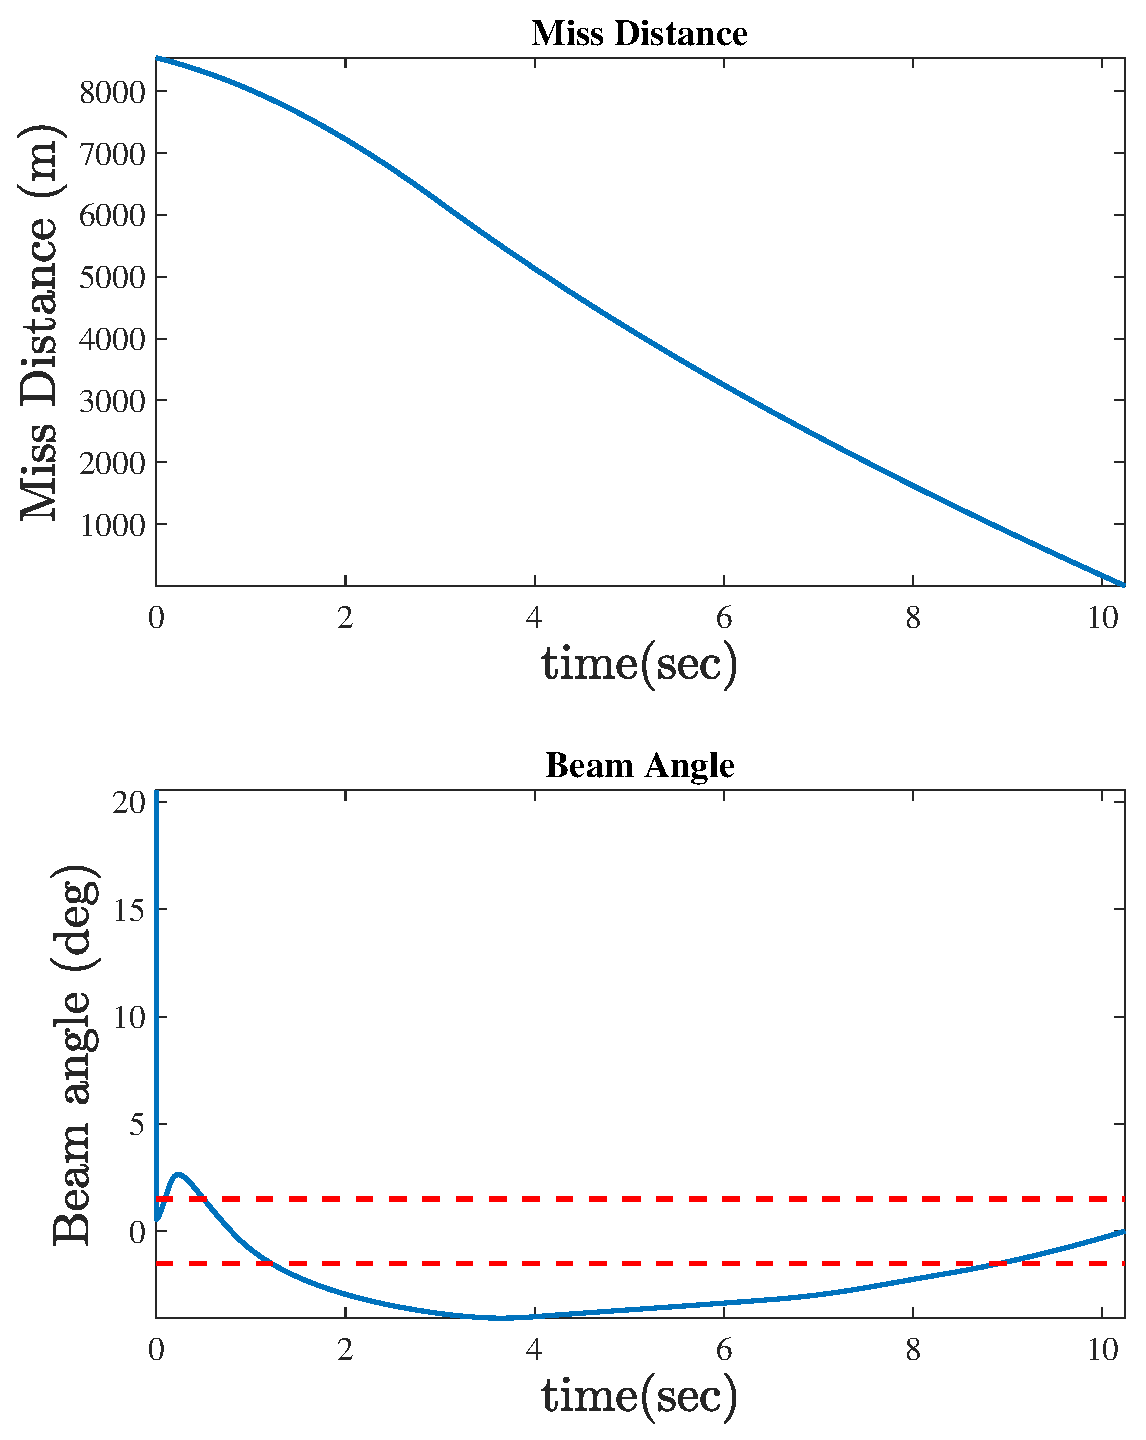
\includegraphics[width=.75\linewidth]{../Figure/k/miss_distance}
	\caption{تاریخچه فاصله ازدست‌دهی و پهنای بیم مورد نیاز در طی مسیر}
\end{figure}
همانطور که در نمودار بالا مشخص است، در بعضی از زمان‌ها از پهنای بیم خارج شده است.